% ******************************* UnB - Departamento de Matemática **************************
% Por favor, dê uma olhada no arquivo LEIAME.md para mais informações sobre como usar o template

\documentclass[a4paper,12pt,times,numbered,index, print]{PhDThesisPSnPDF}

% ******************************************************************************
% ******************************* Opções Comuns ********************************
% *********************** Veja o  LEIAME para mais detalhes ********************
% ******************************************************************************

% `a4paper'(A universidade de Brasília recomenda páginas de tamanho a4 - (opção
% configurada por padrão)

% `oneside' ou `twoside'(padrão): Imprimir em ambos os lados (twoside) ou em um
% lado somente '(oneside)

% `print': Use `print' para configurações próprias à impressão - configurações de
% margem e capítulos. Deixar essa opção em branco ativa a versão Online
% `online': Ativa configurações para versão Online, utilize essa opção para enviar
% seu trabalho à Biblioteca

% `index': Para ativar índice Remissivo ao final da Dissertação

% `draftclassic': Para modo rascunho, sem carregar nenhuma imagem

% `draft': Modo rascunho especial com números de linhas, imagens, e marca d'agua
% com data e texto personalizado. (Veja o arquivo de Prêambulo para configuração)
% IMPORTANTE: Depois de ativado o modo rascunho, ao desativá-lo, o projeto pode
% não compilar. Para resolver este problema basta limpar os arquivos temporários.
% A maioria dos editores de latex já tem esse recurso implementado.

% `chapter`: Use essa opção para ativar somente um capítulo específico e suas referências
%  Útil para correções e revisões

% ********************** Escolhendo estilo de Bibliografia ***********************
%
% `authoryear': Para o formato de autor-ano - ex., Deivid Vale (2018)
%
% `numbered': (Opção Padrão) Para citações enumeradas e ordenadas por nome e.g., [1,5,2]
%
% `custombib': Definir seu próprio estilo de citação no arquivo `preamble.tex'.
%              `\RequirePackage[square, sort, numbers, authoryear]{natbib}'.
%

% ********************************** Preamble **********************************
% Preamble: Configurações somente do template
\input{Preamble/preamble}
% Config: Arquivo de configurações específicas de seu trabalho
% Configure the document math mode and theorems style.

% Comente se o trabalho for escrito em inglês
\usepackage[T1]{fontenc}
\usepackage[utf8]{inputenc}
\usepackage[portuguese]{babel}

%Use this workaround the appendix error with portuguese language
\usepackage{etoolbox}
\makeatletter
\appto{\appendices}{\def\Hy@chapapp{Appendix}}
\makeatother

%Math Packages - General
\usepackage{amsmath,amsthm,amssymb,amsfonts,amscd, amsbsy,mathtools}
\usepackage{mathtools}
\usepackage{wasysym}
\usepackage{xypic}
\CompileMatrices

% Logic
\usepackage{bussproofs}

\everymath{\displaystyle}
\DeclareMathAlphabet{\mathcal}{OMS}{cmsy}{m}{n}
\usepackage{bussproofs}

%Pacotes de Documento
\usepackage{faktor} %Por exemplo, faktor é muito útil para escrever quocientes.
% Para mais informações veja:
% https://ctan.org/pkg/faktor?lang=en


%Ambientes Comuns - Inglês
%\theoremstyle{definition}\newtheorem{definition}{Definition}[chapter]
%\newtheorem{example}{Example}[chapter]
%\newtheorem{lemma}{Lemma}[chapter]
%\newtheorem{theorem}{Theorem}[chapter]
%\newtheorem{proposition}{Proposition}[chapter]
%\newtheorem{col}{Corollary}[chapter]
%\theoremstyle{remark}\newtheorem{remark}{Remark}[chapter]

% Ambientes Comuns - Português
\theoremstyle{definition}\newtheorem{definicao}{Definição}[chapter]
\newtheorem{exemplo}{Exemplo}[chapter]
\newtheorem{lema}{Lema}[chapter]
\newtheorem{teorema}{Teorema}[chapter]
\newtheorem{proposicao}{Proposição}[chapter]
\newtheorem{col}{Corolário}[chapter]
\theoremstyle{remark}\newtheorem{obs}{Observação}[chapter]

% Notation: Arquivo de configuração de comandos de notação. Isso facilita a escrita,
% veja alguns exemplos no arquivo.
%TODO: Make a revision in notation commands, they are very confusing...

% General
\newcommand{\signature}{\Sigma}             %The signature set.
\newcommand{\subs}{\mathcal{S}ub}           %The substitutions set.
\newcommand{\vars}[1]{\mathtt{vars}(#1)}   %The set of variables.
\newcommand{\dom}[1]{\mathtt{dom}(#1)}     %The domain.
\newcommand{\ran}[1]{\mathtt{ran}(#1)}      %The range of a substitution.
\newcommand{\vran}[1]{\mathtt{v}\ran{#1}}

% Nominal Terms and Equality
\newcommand{\atomSet}{\mathbb{A}}           %The set of all atoms.
\newcommand{\var}{\mathbb{X}}               %The set of all META variables.
\newcommand{\abs}[2]{\left[ #1 \right]#2}   %Abstraction term.
\newcommand{\support}[1]{\mathtt{supp}(#1)}          %Support of an permutation.
\newcommand{\permID}{\mathtt{id}}           %Identity permutation.
\newcommand{\pAction}[2]{#1 \cdot #2}       %The action of a permutation on a term.
\newcommand{\pGroup}{\mathbb{P}}            %The group of all permutations acting on the set fo atoms.
\newcommand{\swapping}[2]{(#1 \ \ #2)}      %The Swapping permutation.
\newcommand{\terms}{T(\signature,\atomSet,\var)}    %In context of nominal this is the set of terms.

\newcommand{\fresh}{\#}

\newcommand{\solution}[1]{\mathcal{S}(#1)} %solution set of the problem P
\newcommand{\ueq}[2]{#1\overset{?}{=}#2} %an unification equational problem


%Notation for Equational Unification (general theory)

\newcommand{\sig}[1]{\mathcal{S}ig(#1)} %signature of a set of equations

% #1 The theory, #2 the problem set
\newcommand{\eqSolution}[2]{\mathcal{U}_{#1}(#2)}

%This defines an command with optional arguments
% The arguments are:
%m: mandatory - the theory set of equations name
%g: optional argument - CONVENTION: SEND 1 TO BE TRUE "?" means that the equation is an E-unfication problem
\DeclareDocumentCommand\eqUnif{ m g }{%
	\IfNoValueTF{#2}{=_{#1}}{\overset{?}{=}_{#1}}
}

%This defines an command with optional arguments
% The arguments are: #1 - the theory #2 - the variable set
\DeclareDocumentCommand\iqoless{ O{} O{} }{%
	\precsim_{#1}^{#2}
}
\DeclareDocumentCommand\iqogreater{ O{} O{} }{%
	\succsim_{#1}^{#2}
}
\DeclareDocumentCommand\iqoeq{ O{} O{} }{%
	\simeq_{#1}^{#2}
}

\DeclareDocumentCommand\iqoneq{ O{} O{} }{%
	\npreceq_{#1}^{#2}
}


\DeclareDocumentCommand\csu{ O{}}{%
	\mathcal{U}_{#1}
}

% ************************ Informações da Tese e Meta data **********************
% Não comente esse input, caso contrário a capa do trabalho não funciona direito
% ************************ Informações do Template e Meta-Data **********************
%% Título do Trabalho
\title{Padrão de Dissertação \texorpdfstring{\\ \LaTeX2e}{LaTeX2e}}
%\texorpdfstring é usado para informações de metadata do PDF - use para simplificar símbolos do título na metadata
%\texorpdfstring{LaTeX_Version}{PDF Version (non-latex)} eg.,
%\texorpdfstring{$sigma$}{sigma}

%% Subtítulo (opcional) - comente esta linha se o trabalho não possuir subtítulo
\subtitle{Com Subtítulo}

%% Nome Completo do Autor
\author{Deivid Rodrigues do Vale}

%% Departamento ()
%\dept{Department of Mathematics}
\dept{Departamento de Matemática}

%% Universidade
\university{Universidade de Brasília}
\crest{
\includegraphics[width=1\textwidth]{unb.eps}}


%% Não Altere esta linha
\collegeshield{\includegraphics[width=0.2\textwidth]{CollegeShields/empty_shield.png}}


%% Orientador (opcional)
%% para mútiplos orientadores separe-os com o comando \newline
%\supervisor{Prof. A.B. Co-orientador\newline
%Prof. C.D. Orientador}

%% Nome (na capa) do co-orientador - Supervisor (default) ou deixe abaixo descomentado se seu trabalho for escrito em Português
%% Se o trabalho for em Inglês, simplemente comente a linha abaixo
%\supervisorrole{Co-Orientador: }
%% if no title is desired:
% \supervisorrole{}

%% Supervisor line width: required to align supervisors
%\supervisorlinewidth{0.50\textwidth}

%% Advisor (optional)
%% for multiple advisors, append each advisor with the \newline command
\advisor{Dr. A. Advisor }

%% Advisor Role (optional) - Advisor (default) or leave empty
\advisorrole{Orientador: }
%% if no title is required
% \advisorrole{}

%% Comprimento da linha do nome do Orientador - altere se ficar desalinhado (seu orientador tem um nome muito grande ?)
%\advisorlinewidth{0.50\textwidth}


%% Texto de Submissão, deixe descomentado de acordo com a língua que está escrevendo.
%% Português
\renewcommand{\submissiontext}{Dissertação apresentada como requisito parcial para obtenção do grau de}

%% Inglês
%\renewcommand{\submissiontext}{Dissertation submitted in partial fulfillment of the requirements for the degree of}

%% Nome completo do Grau - Mestre em Matemática (Doutor em Matemática)
\degreetitle{Mestre/Doutor(a) em Matemática}

%% Afiliação do Departamento (opcional)
%\college{Instituto de Ciências Exatas}

%% Submission date
% Default is set as {\monthname[\the\month]\space\the\year}
%\degreedate{September 2014}

%% Meta informação - palavras chave de seu trabalho
\subject{Matemática} \keywords{{LaTeX} {PhD Thesis} {Universidade de Brasília}}


% ***************************** Modo Capítulo ***********************************
% O modo capítulo permite o escritor imprimir um capítulo particular com referências
% Título, Conteúdo, e Frontmatter são desligados por padrão
% Opção útil para revisar um único capítulo ou enviar ao orientador para correções
% Para usar, basta passar a opção `chapter' para a classe do documento

\ifdefineChapter
 \includeonly{Chapter3/chapter3} %escolha qual capítulo deve ser carregado
\fi

% ******************************** Front Matter ********************************
\begin{document}

\frontmatter

\maketitle

\includepdf[pages={{}, 1, {}}]{Assets/second_front}

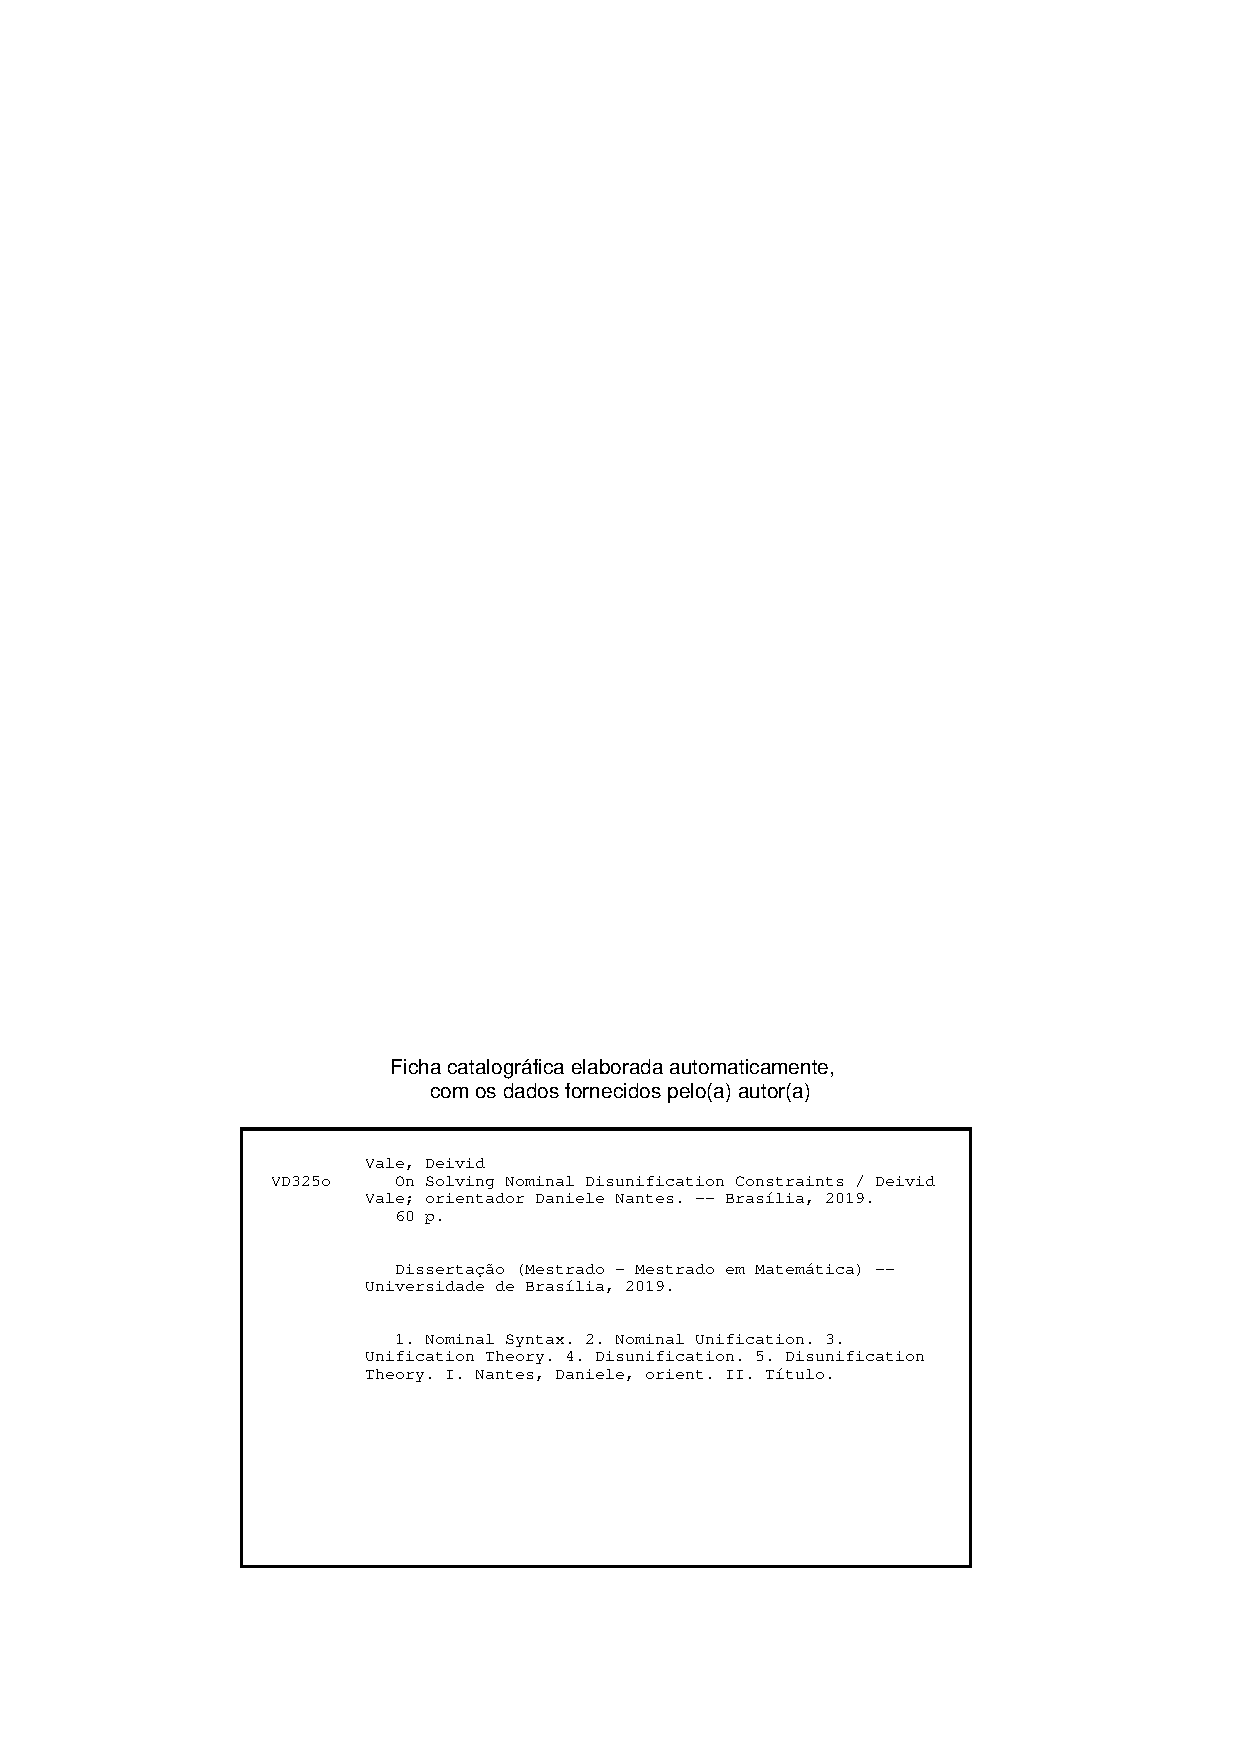
\includepdf[pages={1, {}}]{Assets/library_catalog}

% ******************************* Thesis Dedidcation ********************************

\begin{dedication}
    Dedico este trabalho a...
\end{dedication}


% ************************** Thesis Acknowledgements **************************

\begin{agradecimentos}
    Se a dissertação for escrita em Português.
\end{agradecimentos}

\begin{acknowledgements}
    If the thesis is written in English...
\end{acknowledgements}

% ************************** Thesis Abstract *****************************
% Segundo as regras da Universidade de Brasília, mesmo que a dissertação/tese seja escrita em inglês deve conter um resumo em Português e em Inglês.

\begin{resumo}
    Resumo em Português.
\end{resumo}

\begin{abstract}
This is where you write your abstract ...
\end{abstract}


% *********************** Adding TOC and List of Figures ***********************

\tableofcontents

\listoffigures

\listoftables

% \printnomenclature[space] space can be set as 2em between symbol and description
%\printnomenclature[3em]

\printnomenclature

% ******************************** Main Matter *********************************
\mainmatter

%!TEX root = ../thesis.tex
%*******************************************************************************
%*********************************** First Chapter *****************************
%*******************************************************************************

\chapter*{Introdução}\addcontentsline{toc}{chapter}{Introdução}\markboth{Introdução}{Introdução}

%!TEX root = ../thesis.tex
%*******************************************************************************
%*********************************** First Chapter *****************************
%*******************************************************************************

\chapter*{Introdução}\addcontentsline{toc}{chapter}{Introdução}\markboth{Introdução}{Introdução}

%!TEX root = ../thesis.tex
%*******************************************************************************
%*********************************** First Chapter *****************************
%*******************************************************************************

\chapter*{Introdução}\addcontentsline{toc}{chapter}{Introdução}\markboth{Introdução}{Introdução}

%!TEX root = ../thesis.tex
%*******************************************************************************
%*********************************** First Chapter *****************************
%*******************************************************************************

\chapter*{Introdução}\addcontentsline{toc}{chapter}{Introdução}\markboth{Introdução}{Introdução}

%\include{Chapter4/chapter4}
%\include{Chapter5/chapter5}
%\include{Chapter6/chapter6}
%\include{Chapter7/chapter7}



% ********************************** Back Matter *******************************
% Backmatter should be commented out, if you are using appendices after References
%\backmatter

% ********************************** Bibliography ******************************
\begin{spacing}{0.9}

\bibliographystyle{apalike}
%\bibliographystyle{unsrt} % Use for unsorted references
\cleardoublepage
\bibliography{References/references}

\end{spacing}

% ********************************** Apêndices ********************************

\begin{appendices}

%!TEX root = ../thesis.tex
% ******************************* Thesis Appendix A ****************************
\chapter{Como Instalar o \LaTeX}

\ifpdf
	\graphicspath{{Appendix1/Figs/Raster/}{Appendix1/Figs/PDF/}{Appendix1/Figs/}}
\else
	\graphicspath{{Appendix1/Figs/Vector/}{Appendix1/Figs/}}
\fi

\section*{Windows OS}

Recomendamos o uso do Windows 7 (ou mais novo). Existem dois pacotes de instação do \LaTeX  (mais comuns) o TeXLive e MikTeX. TexLive é mais fácil de trabalhar.

\subsection*{Instalação do TeXLive}
\begin{enumerate}
	\item	Baixe o Intalador do TexLive para windows (link abaixo)\\
	      \href{http://mirror.ctan.org/systems/texlive/tlnet/install-tl-windows.exe}{http://mirror.ctan.org/systems/texlive/tlnet/install-tl-windows.exe}

	\item Para evitar problemas na instalação é recomendado: \textbf{Desligar o Antivírus} e principalmente, \textbf{Executar o Instalador como Administrador}, (Clique com o Botão direito no instalador e escolha a opção \textit{Executar como Administrador}).

	\item O instalador lhe dará três opções de instalação. Primeira, ``Simple Install (big)'' : Instala a maioria dos pacotes, ocupa em torno de 2GB à 4.7GB. Segundo, ``Custom Install'': Instação personalizada e, por último, ``Unpack Only'': somente use essa opção se for realmente preciso e você sabe o que está fazendo.
	\item Se você escolheu a instalação simples no passo acima, apenas aguarde que o processo termine. Isso irá instalar tudo que você precisa para utilizar o \LaTeX.
	\item Passos para instalação customizada:
	      \begin{enumerate}
		      \item Clique no Botão ``Install'' e aguarde um momento até a janela de personalização da instalação ser iniciada. \\
		            \begin{figure}[htbp!]
			            \centering
			            \includegraphics[width=0.7\textwidth]{install-tl-01}
			            \caption[Instação Personalizaa]{Tela Inicial da Instalação Personalizada.}
			            \label{fig:install-tl-01}
                    \end{figure}

              \item Na primeira opção você pode escolher um esquema de instalação. Para compilar a dissertação é recomendado os esquemas: completo ou médio. Você também pode personalizar quais coleções de pacotes deseja instalar. Como na figura abaixo.
              \begin{figure}[htbp!]
                \centering
                \includegraphics[width=0.7\textwidth]{install-tl-02}
                \caption[Instação Personalizaa]{Escolhendo coleções a serem instaladas.}
                \label{fig:install-tl-02}
            \end{figure}

            \item Personalizada a instalação, clique em ``Instalar o TeXLive'' e espere todos os downloads terminarem.
	      \end{enumerate}
\end{enumerate}


\subsection*{Basic MikTeX - \TeX~ distribution}
\begin{enumerate}
	\item	Download Basic-MiK\TeX (32bit or 64bit) from\\
	      \href{http://miktex.org/download}{http://miktex.org/download}
	\item	Run the installer
	\item	To add a new package go to Start >> All Programs >> MikTex >> Maintenance (Admin) and choose Package Manager
	\item	Select or search for packages to install
\end{enumerate}

\section*{Editor - \TeX~ }
Existem vários editores para \LaTeX, escolha o que você mais gosta. Recomendados:
\begin{enumerate}
	\item \textbf{TexStudio}: editor poderoso e fácil de usar, pode ser baixado do link abaixo\\
	      \href{https://www.texstudio.org/}{https://www.texstudio.org/}
        \begin{enumerate}
            \item	Execute o Instalador
	        \item (Opcional): Você pode instalar o \textbf{Language Tool}\footnote{Necessário possuir Java 8 ou superior.} para suporte à correções gramaticais e de estilo linguístico. Baixe o Language tool no endereço \\
            \href{https://languagetool.org/pt}{https://languagetool.org/pt}
        \end{enumerate}

    \item \textbf{Visual Studio Code:} É um editor de objetivo geral, mas pode ser utilizado de maneira muito simples para edição de documetos \LaTeX. Baixe em \\
    \href{https://code.visualstudio.com}{https://code.visualstudio.com}

    \begin{enumerate}
        \item O Suporte \LaTeX para o Visual Studio Code é instalado por uma extenção (\href{https://marketplace.visualstudio.com/items?itemName=James-Yu.latex-workshop}{\textbf{Latex Workshop}}). Basta seguir as instruções em \href{https://marketplace.visualstudio.com/items?itemName=James-Yu.latex-workshop}{neste link.}
    \end{enumerate}


\end{enumerate}

\section*{Mac OS X}
\subsection*{MacTeX - \TeX~ distribuição}
\begin{enumerate}
	\item	Baixe o instalador de\\
	      \href{https://www.tug.org/mactex/}{https://www.tug.org/mactex/}
	\item	Extraia e execute o instalador. A configuração é automática.
\end{enumerate}

\section*{Unix/Linux}

\subsubsection*{Fedora/RedHat/CentOS:}
\begin{verbatim}
sudo yum install texlive
sudo yum install psutils
\end{verbatim}


\subsubsection*{SUSE:}
\begin{verbatim}
sudo zypper install texlive
\end{verbatim}


\subsubsection*{Debian/Ubuntu:}
\begin{verbatim}
sudo apt-get install texlive-full
sudo apt-get install psutils
\end{verbatim}


\end{appendices}

% *************************************** Index ********************************
\printthesisindex % If index is present

\end{document}
